\documentclass[11pt,a4paper]{article}

% --- Packages ---
\usepackage[utf8]{inputenc}
\usepackage[T1]{fontenc}
\usepackage{lmodern}
\usepackage[margin=2.5cm]{geometry}
\usepackage{graphicx}
\usepackage{booktabs}
\usepackage{amsmath,amssymb}
\usepackage{xcolor}
\usepackage{hyperref}
\usepackage{caption}
\usepackage{subcaption}
\usepackage{float}
\usepackage{enumitem}
\usepackage{siunitx}

\hypersetup{
    colorlinks=true,
    linkcolor=blue!60!black,
    citecolor=blue!60!black,
    urlcolor=blue!60!black,
}

% Path to figures
\graphicspath{
    {../outputs/baseline/evaluate/}
    {../outputs/improved/evaluate/}
    {../outputs/ablation/}
}

\title{%
    \textbf{Flow Matching for Predictive Time-Series Forecasting:}\\[4pt]
    \Large Overcoming Latency in High-Frequency Systems\\[12pt]
    \large Section~4 --- Experiments and Results
}
\author{
    Ka Wong Hui \and Min-Han Yeh
}
\date{March 2026}

\begin{document}
\maketitle

% ==============================================================================
\section{Experiments and Results}
% ==============================================================================

% ------------------------------------------------------------------------------
\subsection{Experimental Setup}
\label{sec:setup}
\textit{(Main Author: Ka Wong Hui)}

\subsubsection{Dataset}

All experiments use the CWRU Bearing Fault Dataset at
\SI{12000}{samples\per\second} (Drive End accelerometer).
Four operating conditions are included: Normal, Inner Race fault (IR007),
Ball fault (B007), and Outer Race fault (OR007).
Each signal is segmented into sliding windows with a context length of
256~timesteps and a prediction horizon of 64~timesteps, using a stride of~64.

The dataset is split \emph{per fault condition} on the raw signal timeline to
prevent data leakage: 70\% training, 15\% validation, 15\% test.
This yields 6{,}652 training windows, 1{,}408 validation windows, and
1{,}410 test windows.
Normalization statistics ($z$-score) are computed on the training split only.

\subsubsection{Model Architecture}

Both models use an identical TCN velocity field with 6~layers,
256~hidden channels, kernel size~3, dropout~0.2, and a 64-dimensional
sinusoidal time embedding.
Both models have exactly \textbf{2{,}615{,}233 trainable parameters},
ensuring any performance difference is attributable to the Flow Matching
formulation, not model capacity.

\subsubsection{Training Configuration}

\begin{table}[H]
\centering
\caption{Training hyperparameters (shared by both models).}
\label{tab:training-config}
\begin{tabular}{@{}ll@{}}
\toprule
\textbf{Parameter} & \textbf{Value} \\
\midrule
Optimizer           & AdamW ($\text{lr}=5\times10^{-4}$, weight decay $=1\times10^{-5}$) \\
LR schedule         & Linear warmup (10 epochs) $+$ cosine annealing ($T_{\max}=500$) \\
Batch size          & 128 \\
Gradient clipping   & Max norm 1.0 \\
Mixed precision     & Enabled (\texttt{torch.cuda.amp}) \\
Early stopping      & Patience $=30$ eval rounds (eval every 5 epochs) \\
Max epochs          & 500 \\
Hardware            & NVIDIA GPU with \texttt{torch.compile} (reduce-overhead) \\
\bottomrule
\end{tabular}
\end{table}

\subsubsection{Evaluation Protocol}

Both models are evaluated with \textbf{30 Monte Carlo samples} per test
window.
At each test input the model generates 30 independent stochastic forecasts
by sampling different initial noise and solving the probability-flow ODE.
Metrics are computed as follows:

\begin{itemize}[nosep]
    \item \textbf{MAE / RMSE} --- computed on the mean of the 30 samples
          versus ground truth.
    \item \textbf{CRPS} --- empirical Continuous Ranked Probability Score
          measuring probabilistic calibration
          ($\text{CRPS} = \mathbb{E}|X-y| - \tfrac{1}{2}\mathbb{E}|X-X'|$).
    \item \textbf{P10--P90 Coverage} --- fraction of true values falling
          within the 10th--90th percentile interval of the 30 samples
          (ideal $\approx 80\%$).
    \item \textbf{Latency} --- single-sample wall-clock inference time
          averaged over 100~iterations after 10~warmup iterations.
\end{itemize}

The baseline is evaluated at its design operating point of \textbf{NFE\,=\,16},
and the improved model at \textbf{NFE\,=\,4}, as hypothesized in the proposal.

% ------------------------------------------------------------------------------
\subsection{Objective Results}

% --- 4.2.1 Training Dynamics ---
\subsubsection{Training Dynamics}
\label{sec:training-dynamics}
\textit{(Main Author: Ka Wong Hui)}

\begin{figure}[H]
\centering
\begin{subfigure}[t]{0.48\textwidth}
    \centering
    
\includegraphics[width=\textwidth]{training_loss.png}
    \caption{Baseline model --- widening train/val gap indicates overfitting
             after $\sim$50 epochs.}
    \label{fig:loss-baseline}
\end{subfigure}
\hfill
\begin{subfigure}[t]{0.48\textwidth}
    \centering
    
\includegraphics[width=\textwidth]{training_loss.png}
    \caption{Improved model --- train and val losses remain tightly coupled
             throughout 500~epochs.}
    \label{fig:loss-improved}
\end{subfigure}
\caption{Training progress for both models (log scale).}
\label{fig:training-loss}
\end{figure}

The two models exhibit markedly different training behavior:

\paragraph{Baseline model.}
Training converged rapidly, reaching a best validation loss of
\textbf{0.3674} at epoch~110.
A widening gap between training loss ($\sim$0.28) and validation loss
($\sim$0.39--0.43) is clearly visible from epoch~50 onward
(Figure~\ref{fig:loss-baseline}).
Early stopping triggered at epoch~260 after 30~consecutive evaluation
rounds without improvement.

\paragraph{Improved model.}
Training and validation losses tracked each other closely throughout all
500~epochs, converging to a best validation loss of \textbf{0.0491}
(Figure~\ref{fig:loss-improved}).
No significant overfitting gap developed and training was not early-stopped.

\medskip
\noindent\textbf{Note:} The absolute loss values between the two models are
\emph{not directly comparable}.
The baseline computes the Flow Matching loss against Gaussian
$\mathcal{N}(\mathbf{0},\mathbf{I})$ source samples, while the improved model
uses OU process samples that are already temporally structured.
The OU prior produces velocity targets of inherently smaller magnitude,
resulting in lower loss values.
The overfitting pattern in the baseline, however, is a meaningful finding
independent of the loss scale.

% --- 4.2.2 Accuracy Comparison ---
\subsubsection{Predictive Accuracy --- Baseline vs.\ Improved}
\label{sec:accuracy}
\textit{(Main Author: Min-Han Yeh)}

\begin{table}[H]
\centering
\caption{Primary comparison at design operating points
         (normalized scale, 30 Monte Carlo samples).}
\label{tab:primary}
\begin{tabular}{@{}lccc@{}}
\toprule
\textbf{Metric} & \textbf{Baseline (NFE=16)} & \textbf{Improved (NFE=4)} & $\boldsymbol{\Delta}$ \\
\midrule
MAE              & 0.2793  & 0.2817  & $+0.9\%$   \\
RMSE             & 0.6540  & 0.6366  & $\mathbf{-2.7\%}$  \\
CRPS             & 0.2098  & 0.2267  & $+8.1\%$   \\
P10--P90 Coverage & 58.5\% & 40.5\%  & $-18.0$\,pp \\
Mean Pred.\ Std  & 0.197   & 0.131   & $-33.8\%$  \\
Latency          & \SI{71.0}{\milli\second} & \SI{21.7}{\milli\second} & $\mathbf{-69.4\%}$ \\
\bottomrule
\end{tabular}
\end{table}

\begin{table}[H]
\centering
\caption{Comparison on original scale (before $z$-score normalization).}
\label{tab:original-scale}
\begin{tabular}{@{}lcc@{}}
\toprule
\textbf{Metric} & \textbf{Baseline (NFE=16)} & \textbf{Improved (NFE=4)} \\
\midrule
MAE  & 0.0938 & 0.0945 \\
RMSE & 0.2195 & 0.2137 \\
\bottomrule
\end{tabular}
\end{table}

\noindent Key findings:

\begin{enumerate}[nosep]
    \item \textbf{Point accuracy is competitive.}
          The improved model at 4~NFEs achieves MAE within 0.9\% and RMSE
          2.7\% \emph{better} than the baseline at 16~NFEs---broadly
          confirming the hypothesis.
    \item \textbf{Inference speed improved $\mathbf{3.3\times}$.}
          Latency dropped from \SI{71.0}{\milli\second} to
          \SI{21.7}{\milli\second}.
          While neither meets the sub-millisecond target stated in the
          proposal (which would require hardware-level optimizations beyond
          this project's scope), the relative improvement is substantial.
    \item \textbf{Uncertainty calibration is a trade-off.}
          The improved model's P10--P90 coverage of 40.5\% is significantly
          below the baseline's 58.5\% and the ideal 80\%.
          The prediction intervals are too narrow, indicating overconfident
          uncertainty estimates.
\end{enumerate}

% --- Forecast examples ---
\begin{figure}[H]
\centering
\begin{subfigure}[t]{0.48\textwidth}
    \centering
    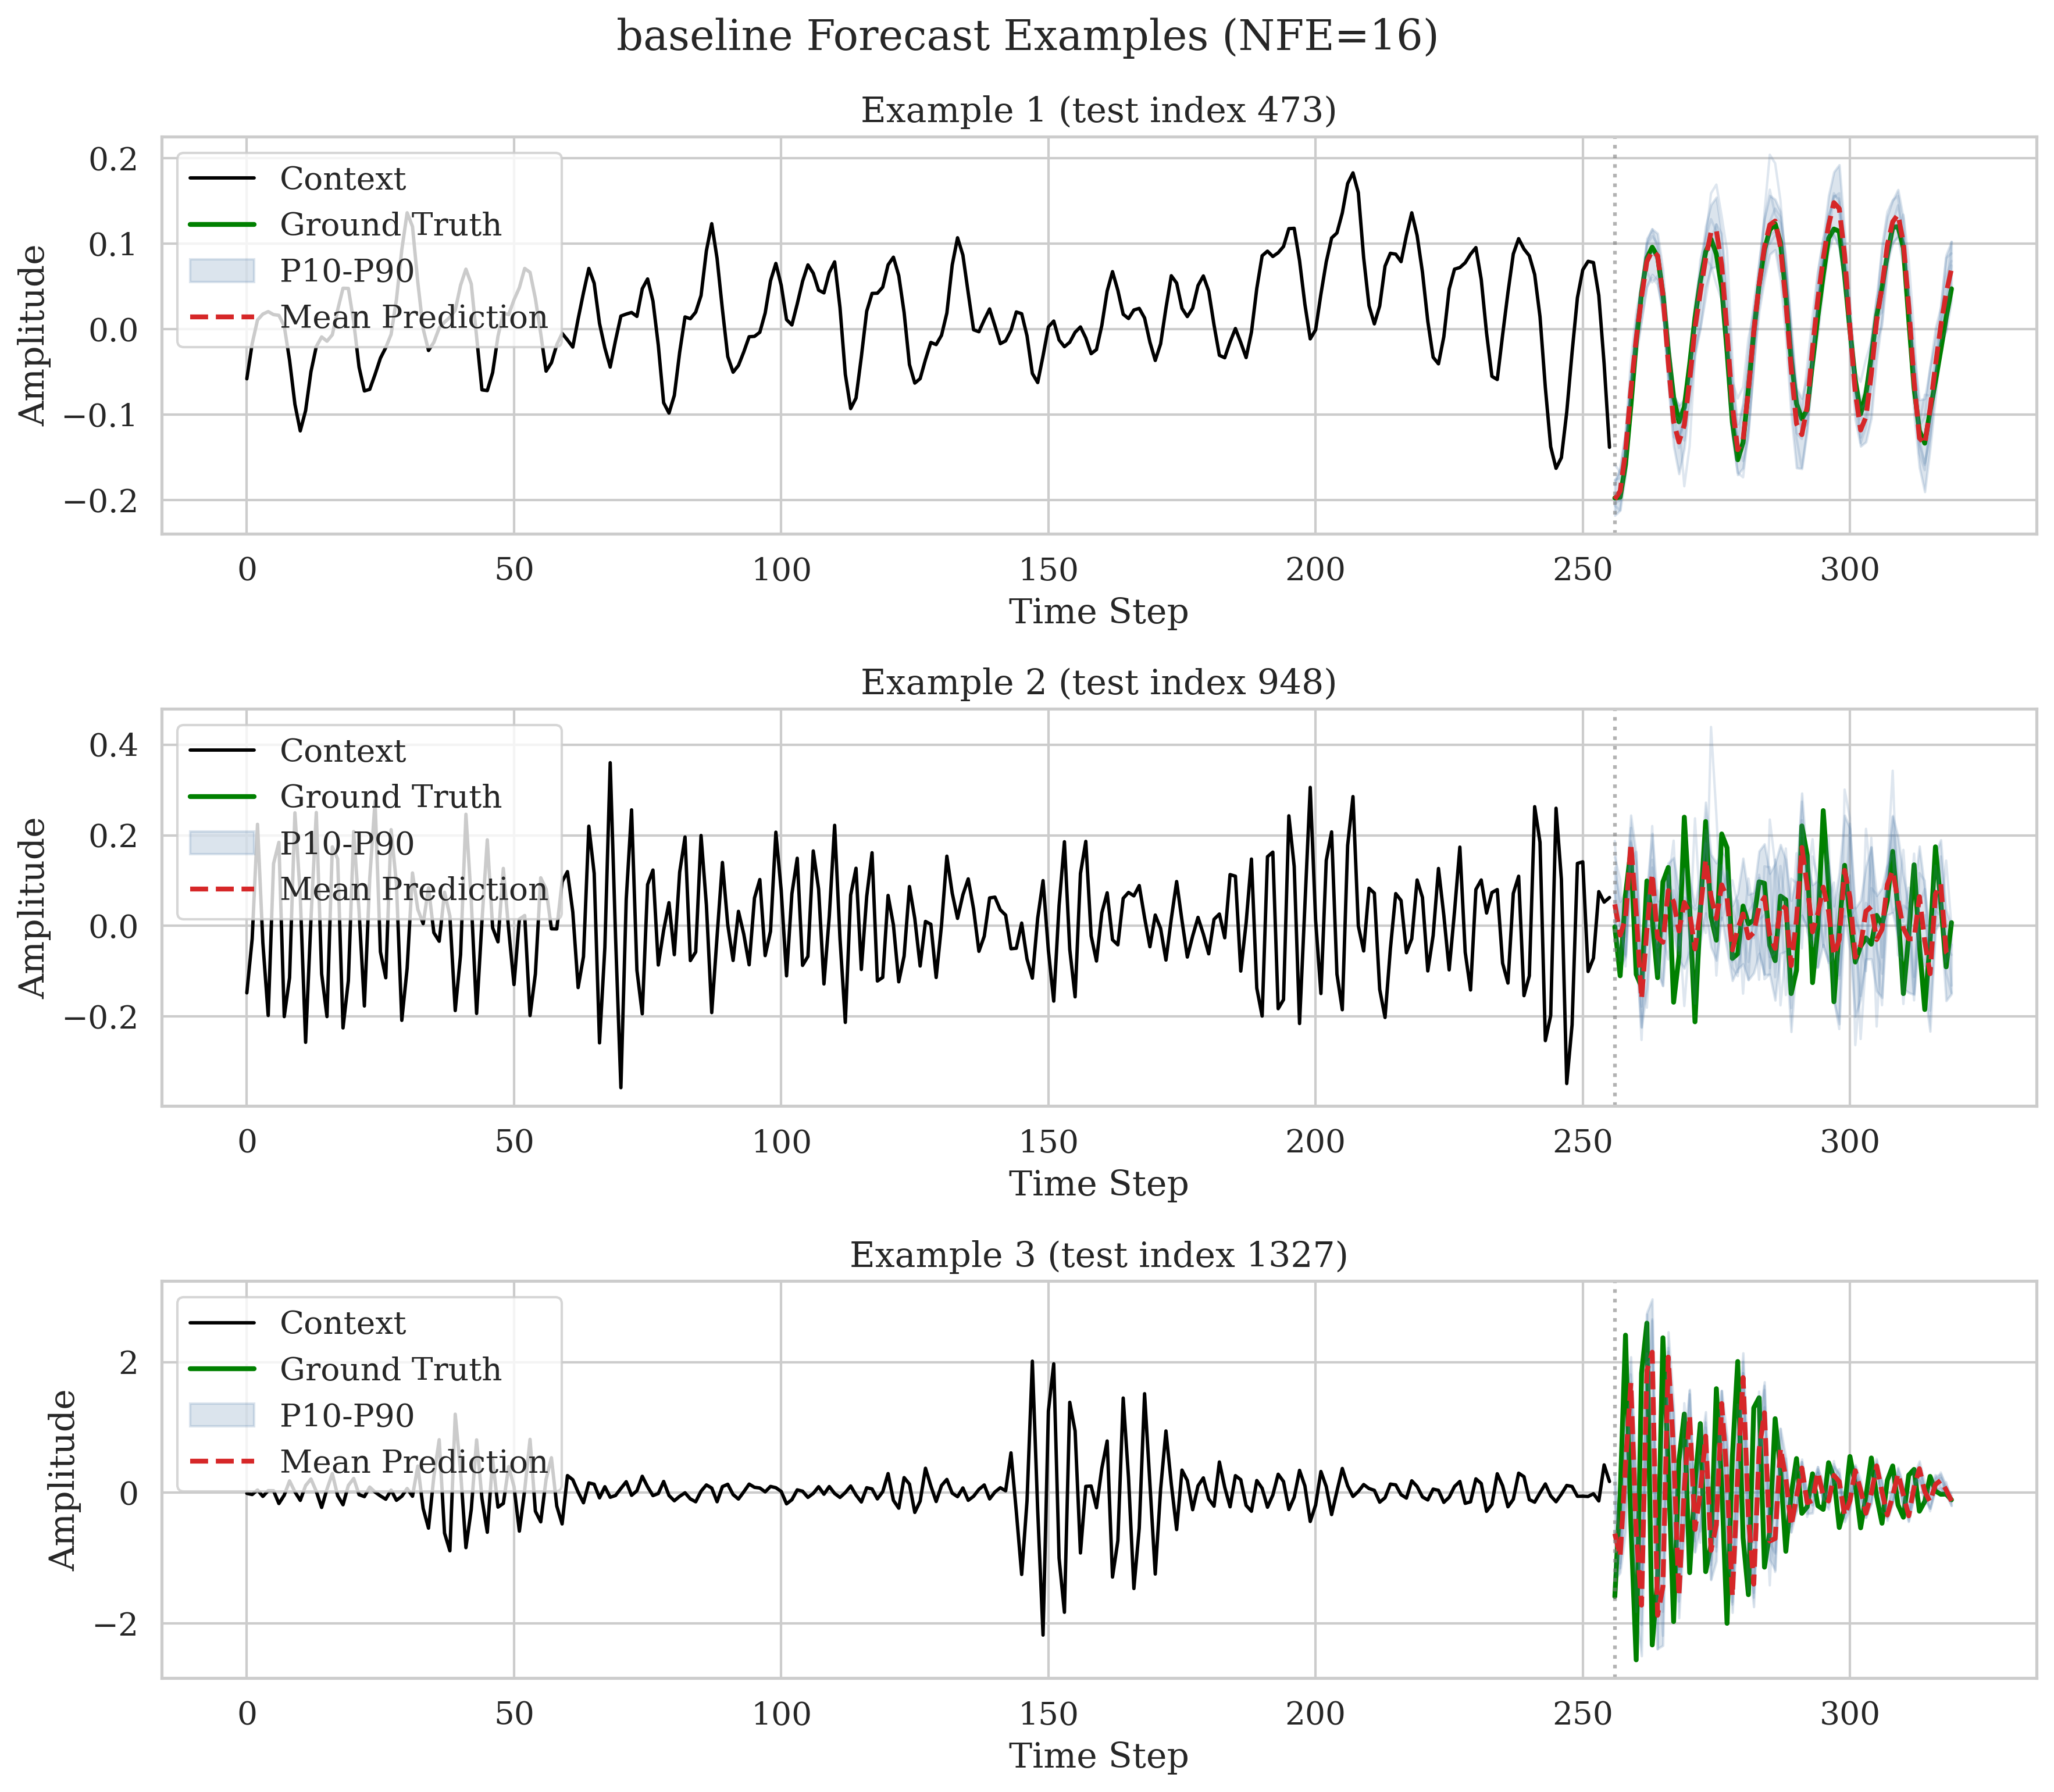
\includegraphics[width=\textwidth]{forecast_examples_nfe16.png}
    \caption{Baseline (NFE\,=\,16).}
\end{subfigure}
\hfill
\begin{subfigure}[t]{0.48\textwidth}
    \centering
    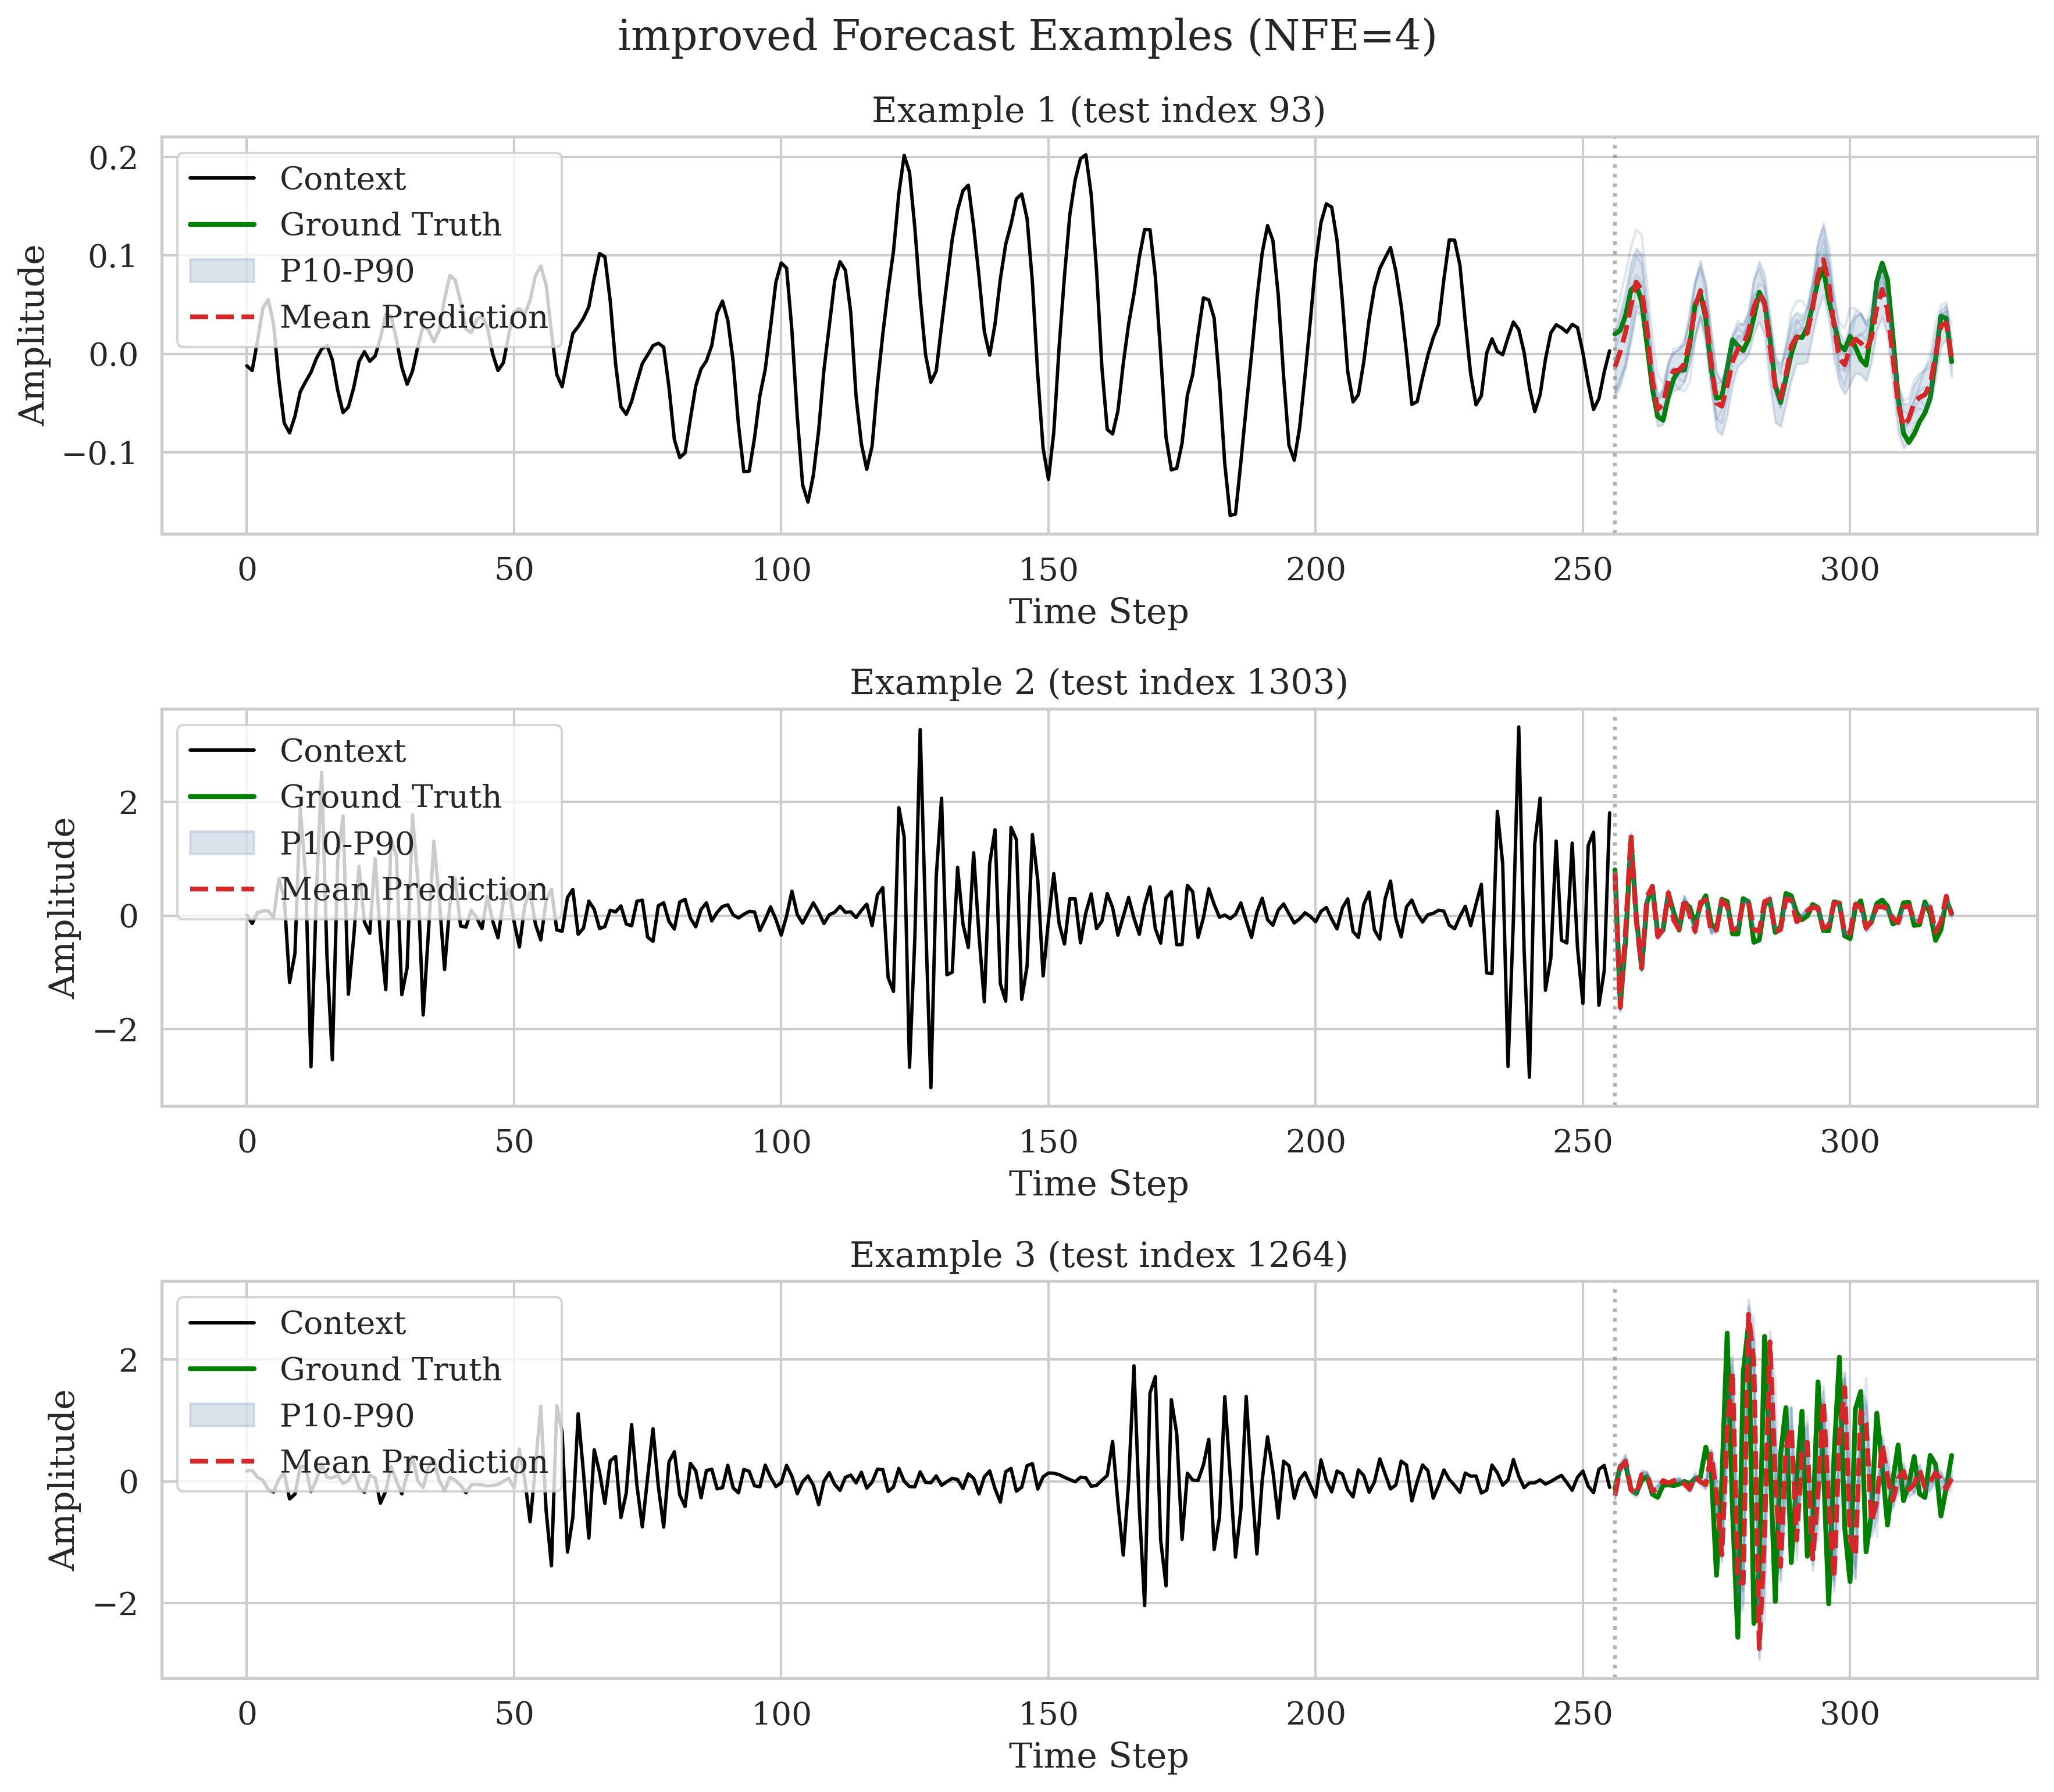
\includegraphics[width=\textwidth]{forecast_examples_nfe4.png}
    \caption{Improved (NFE\,=\,4) --- note the narrower P10--P90 bands.}
\end{subfigure}
\caption{Representative forecast examples at low-, medium-, and high-error
         quantiles of the test set.}
\label{fig:forecasts}
\end{figure}

% --- Error by horizon ---
\begin{figure}[H]
\centering
\begin{subfigure}[t]{0.48\textwidth}
    \centering
    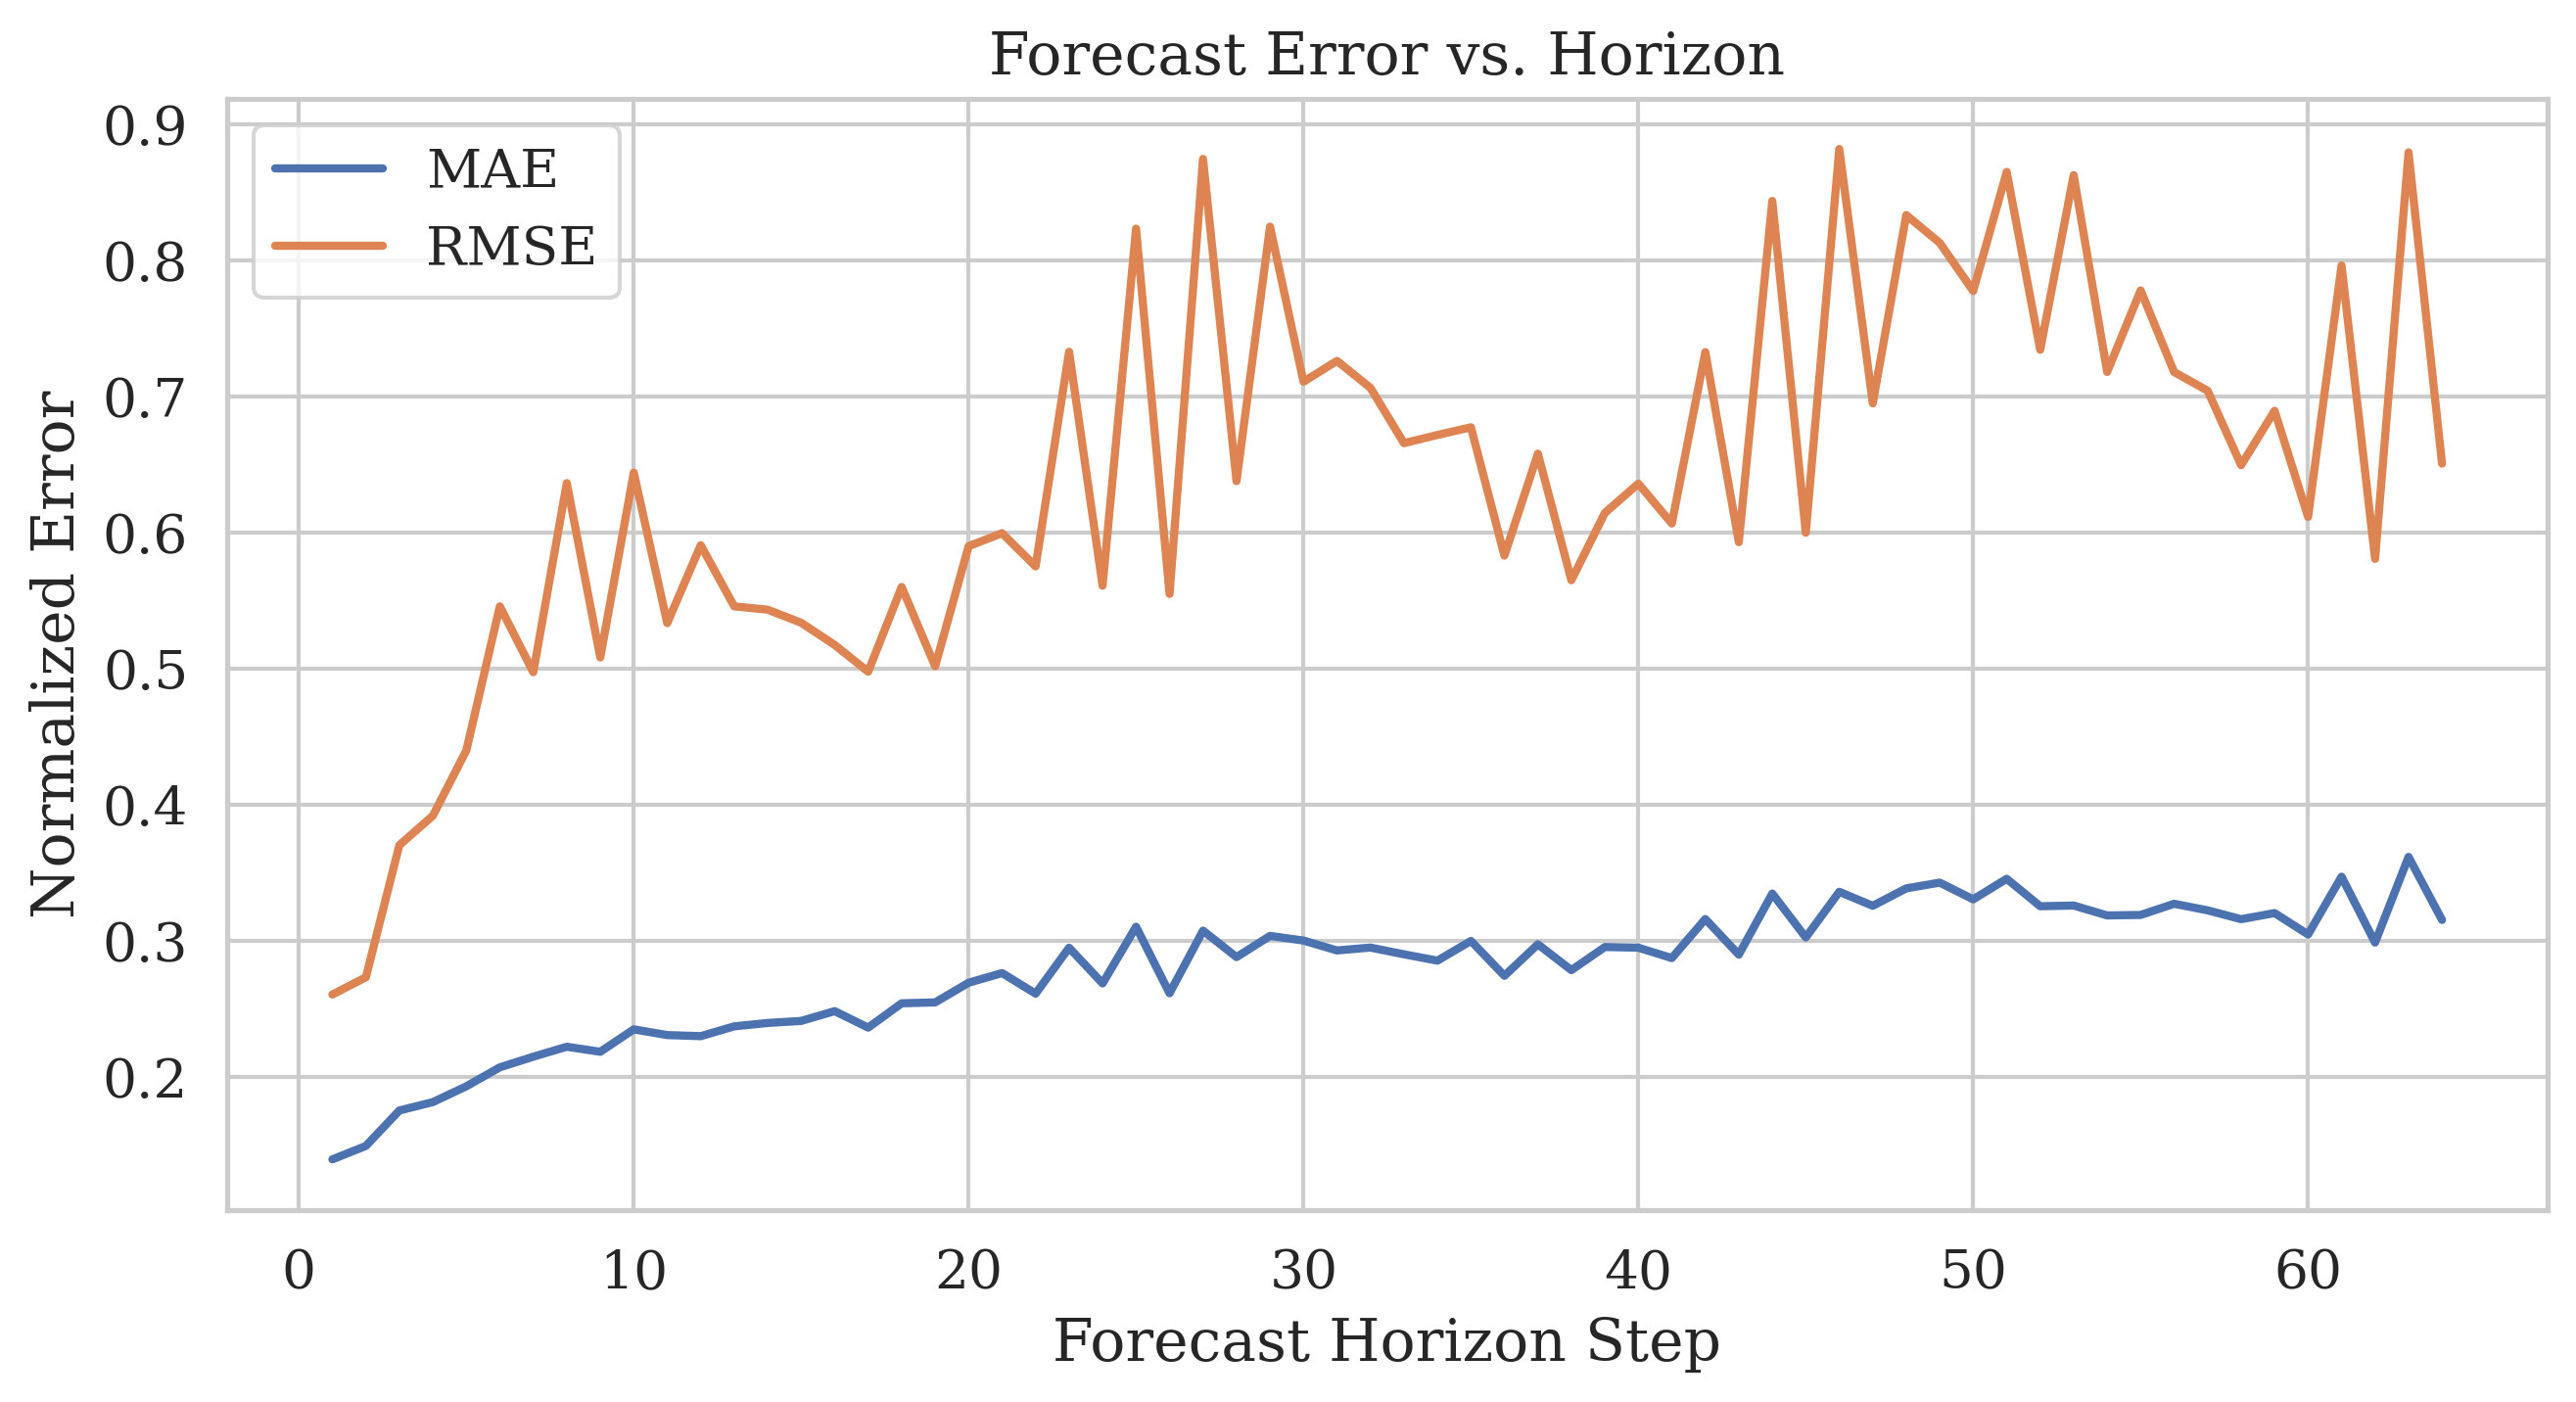
\includegraphics[width=\textwidth]{error_by_horizon_nfe16.png}
    \caption{Baseline (NFE\,=\,16).}
\end{subfigure}
\hfill
\begin{subfigure}[t]{0.48\textwidth}
    \centering
    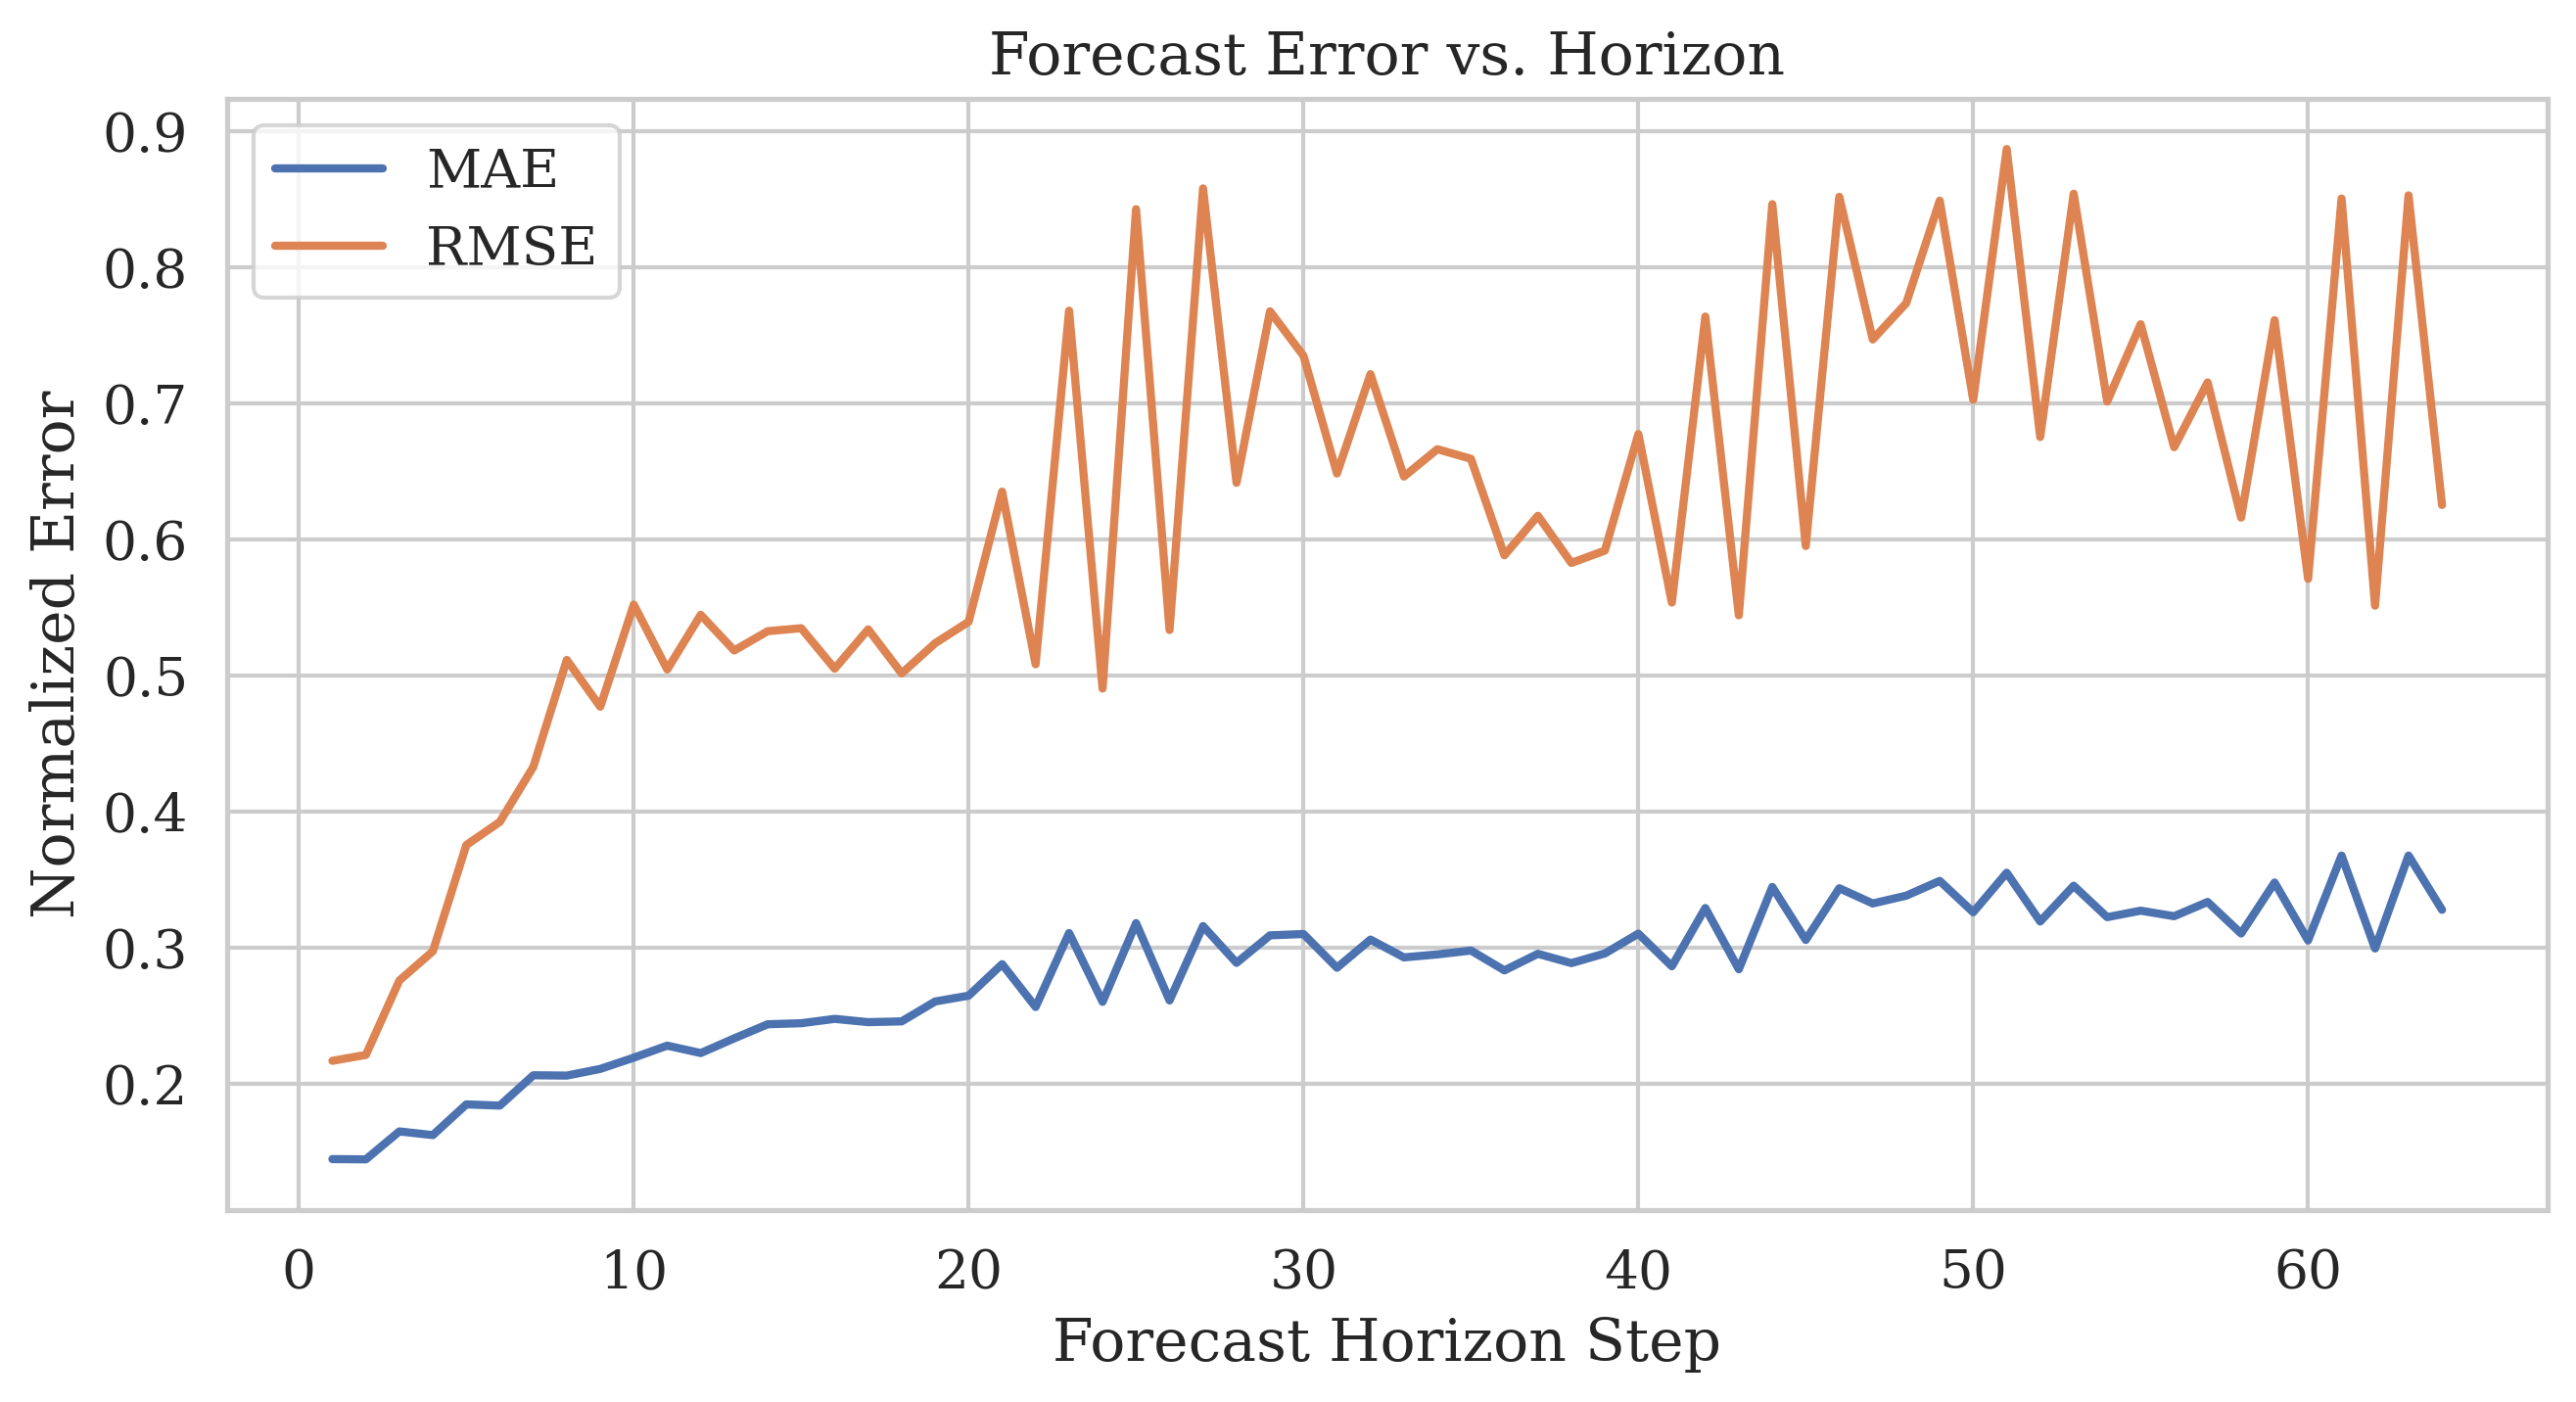
\includegraphics[width=\textwidth]{error_by_horizon_nfe4.png}
    \caption{Improved (NFE\,=\,4).}
\end{subfigure}
\caption{MAE and RMSE growth across the 64-step forecast horizon.
         Both models show comparable error growth rates, indicating the
         improved model's advantage is consistent across the entire
         prediction window.}
\label{fig:horizon-error}
\end{figure}

% --- 4.2.3 Ablation ---
\subsubsection{NFE Ablation Study}
\label{sec:ablation}
\textit{(Main Author: Min-Han Yeh)}

To rigorously evaluate the accuracy--latency trade-off, both models are
evaluated across NFE\,$\in\{2, 4, 8, 16, 32\}$ with 64~Monte Carlo samples
per test window.

\begin{table}[H]
\centering
\caption{NFE ablation results (normalized MAE and single-sample latency).}
\label{tab:ablation}
\begin{tabular}{@{}rcccc@{}}
\toprule
\textbf{NFE}
  & \textbf{Baseline MAE} & \textbf{Improved MAE}
  & \textbf{Baseline Lat.\ (ms)} & \textbf{Improved Lat.\ (ms)} \\
\midrule
 2  & 0.2846 & 0.2861 &   7.3 &  14.2 \\
 4  & 0.2800 & 0.2816 &  13.9 &  21.2 \\
 8  & 0.2783 & 0.2782 &  27.8 &  35.1 \\
16  & 0.2780 & 0.2762 &  55.6 &  64.3 \\
32  & 0.2790 & 0.2758 & 111.3 & 119.6 \\
\bottomrule
\end{tabular}
\end{table}

\begin{figure}[H]
\centering
\begin{subfigure}[t]{0.48\textwidth}
    \centering
    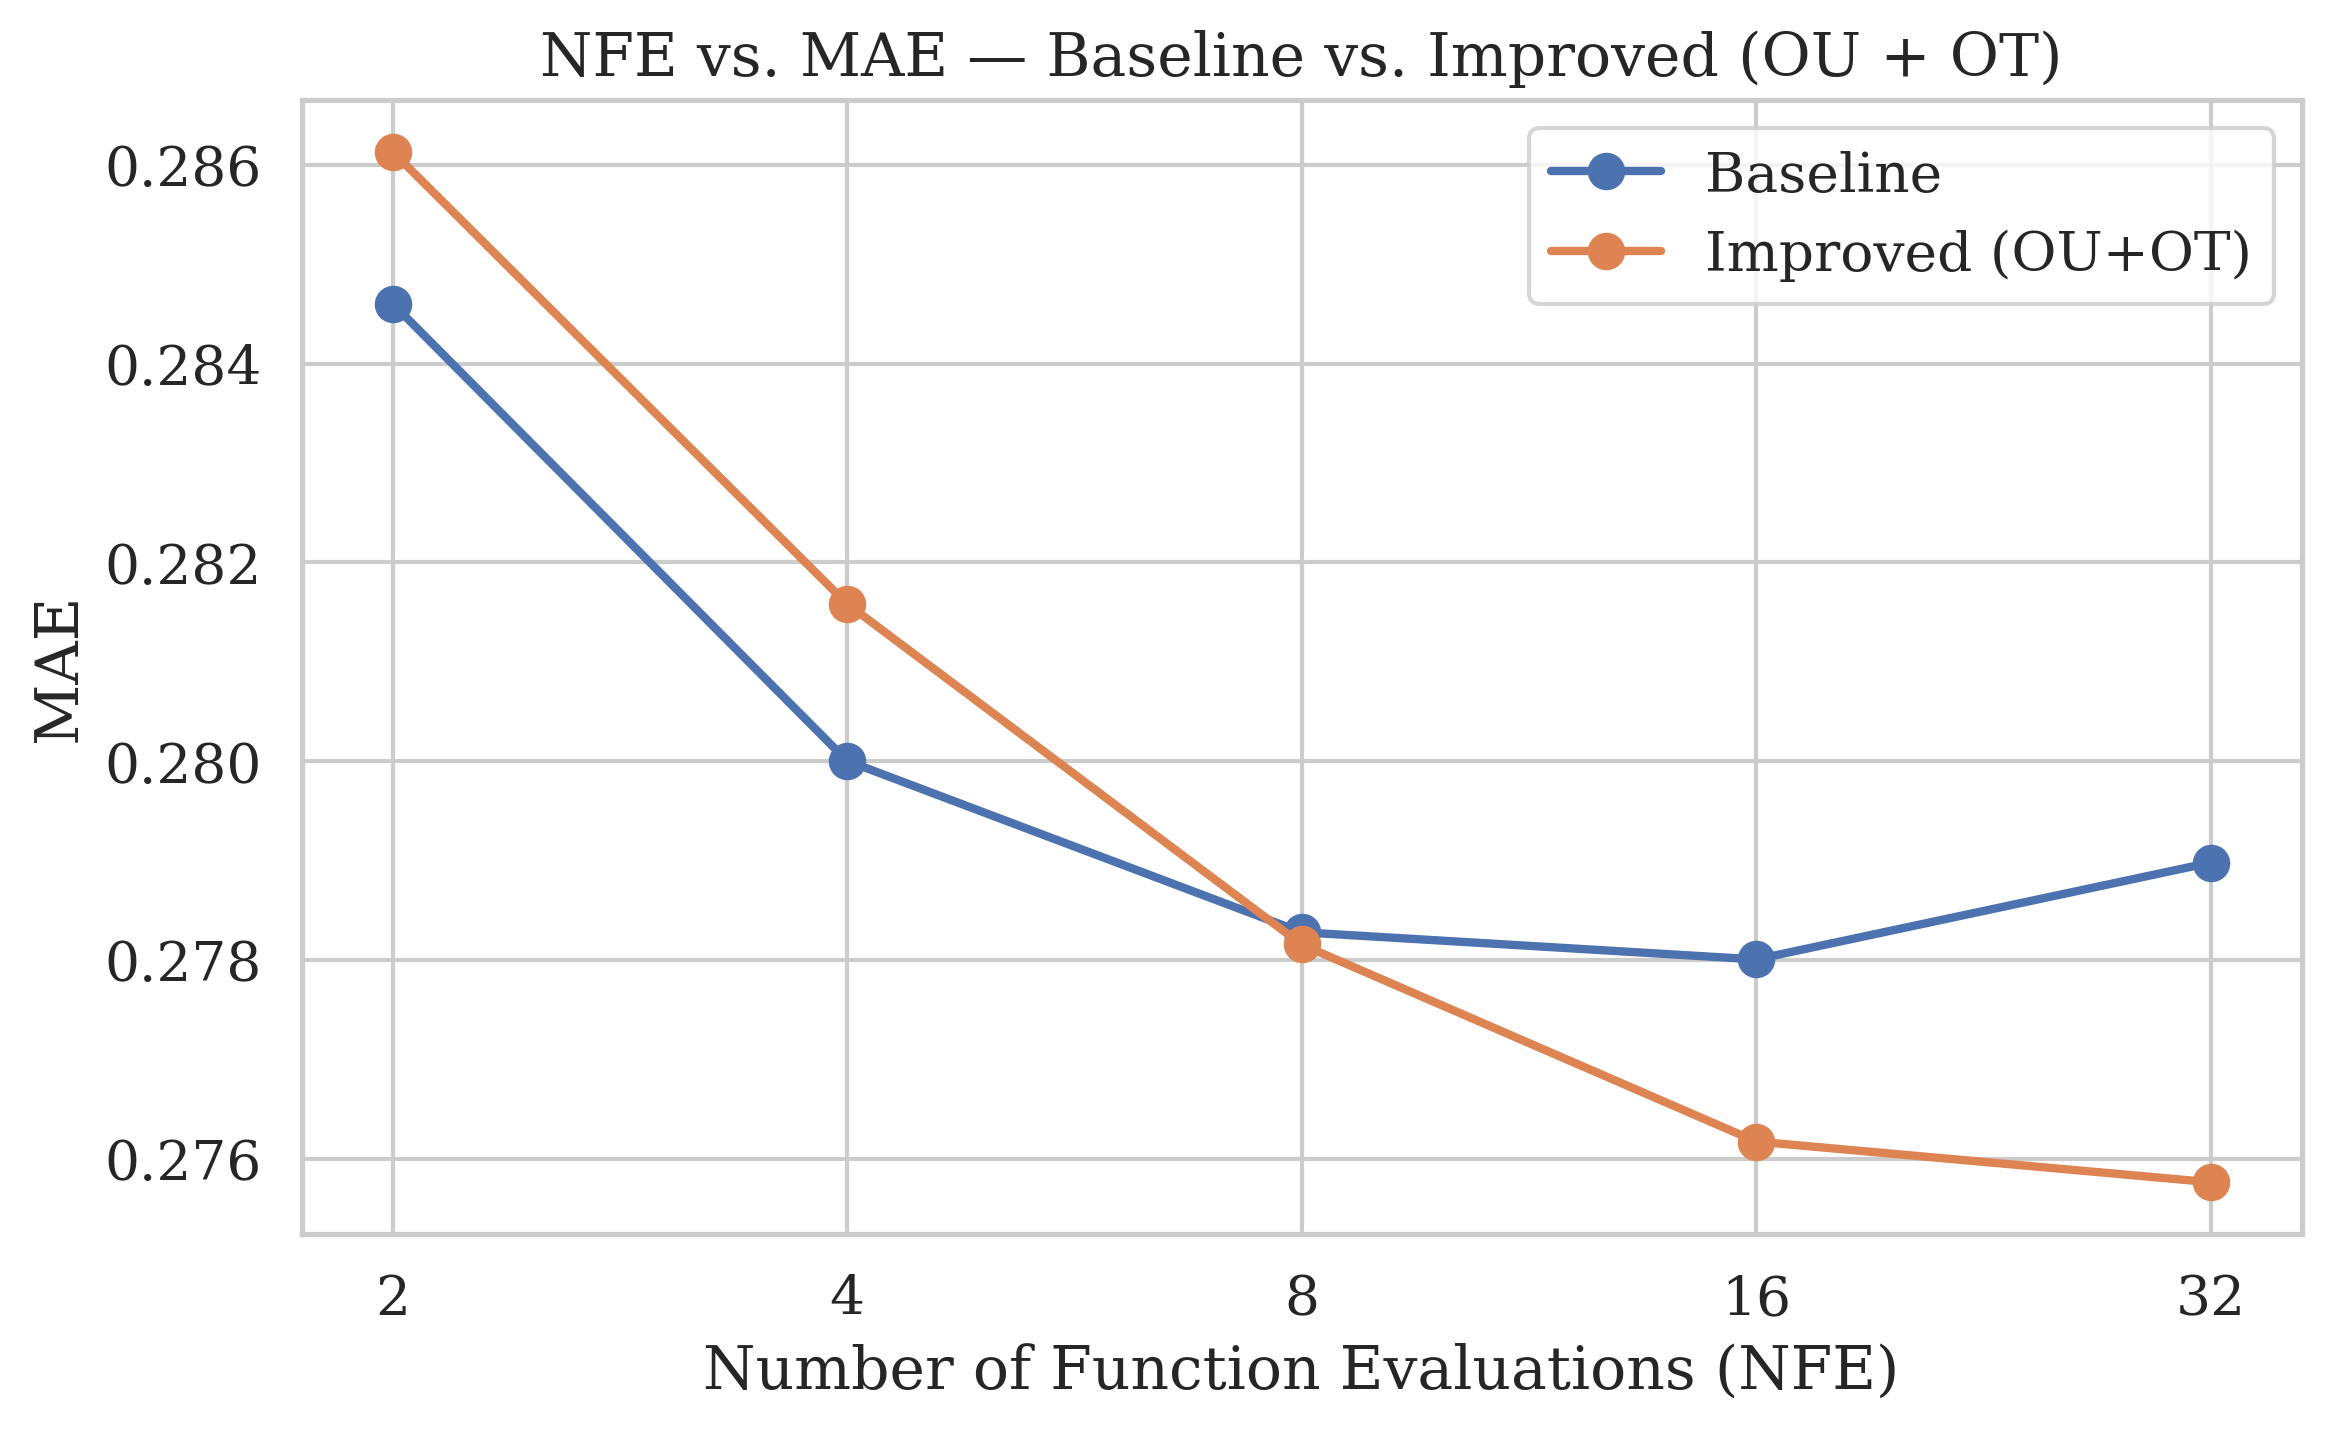
\includegraphics[width=\textwidth]{nfe_vs_mae.png}
    \caption{NFE vs.\ MAE.}
    \label{fig:nfe-mae}
\end{subfigure}
\hfill
\begin{subfigure}[t]{0.48\textwidth}
    \centering
    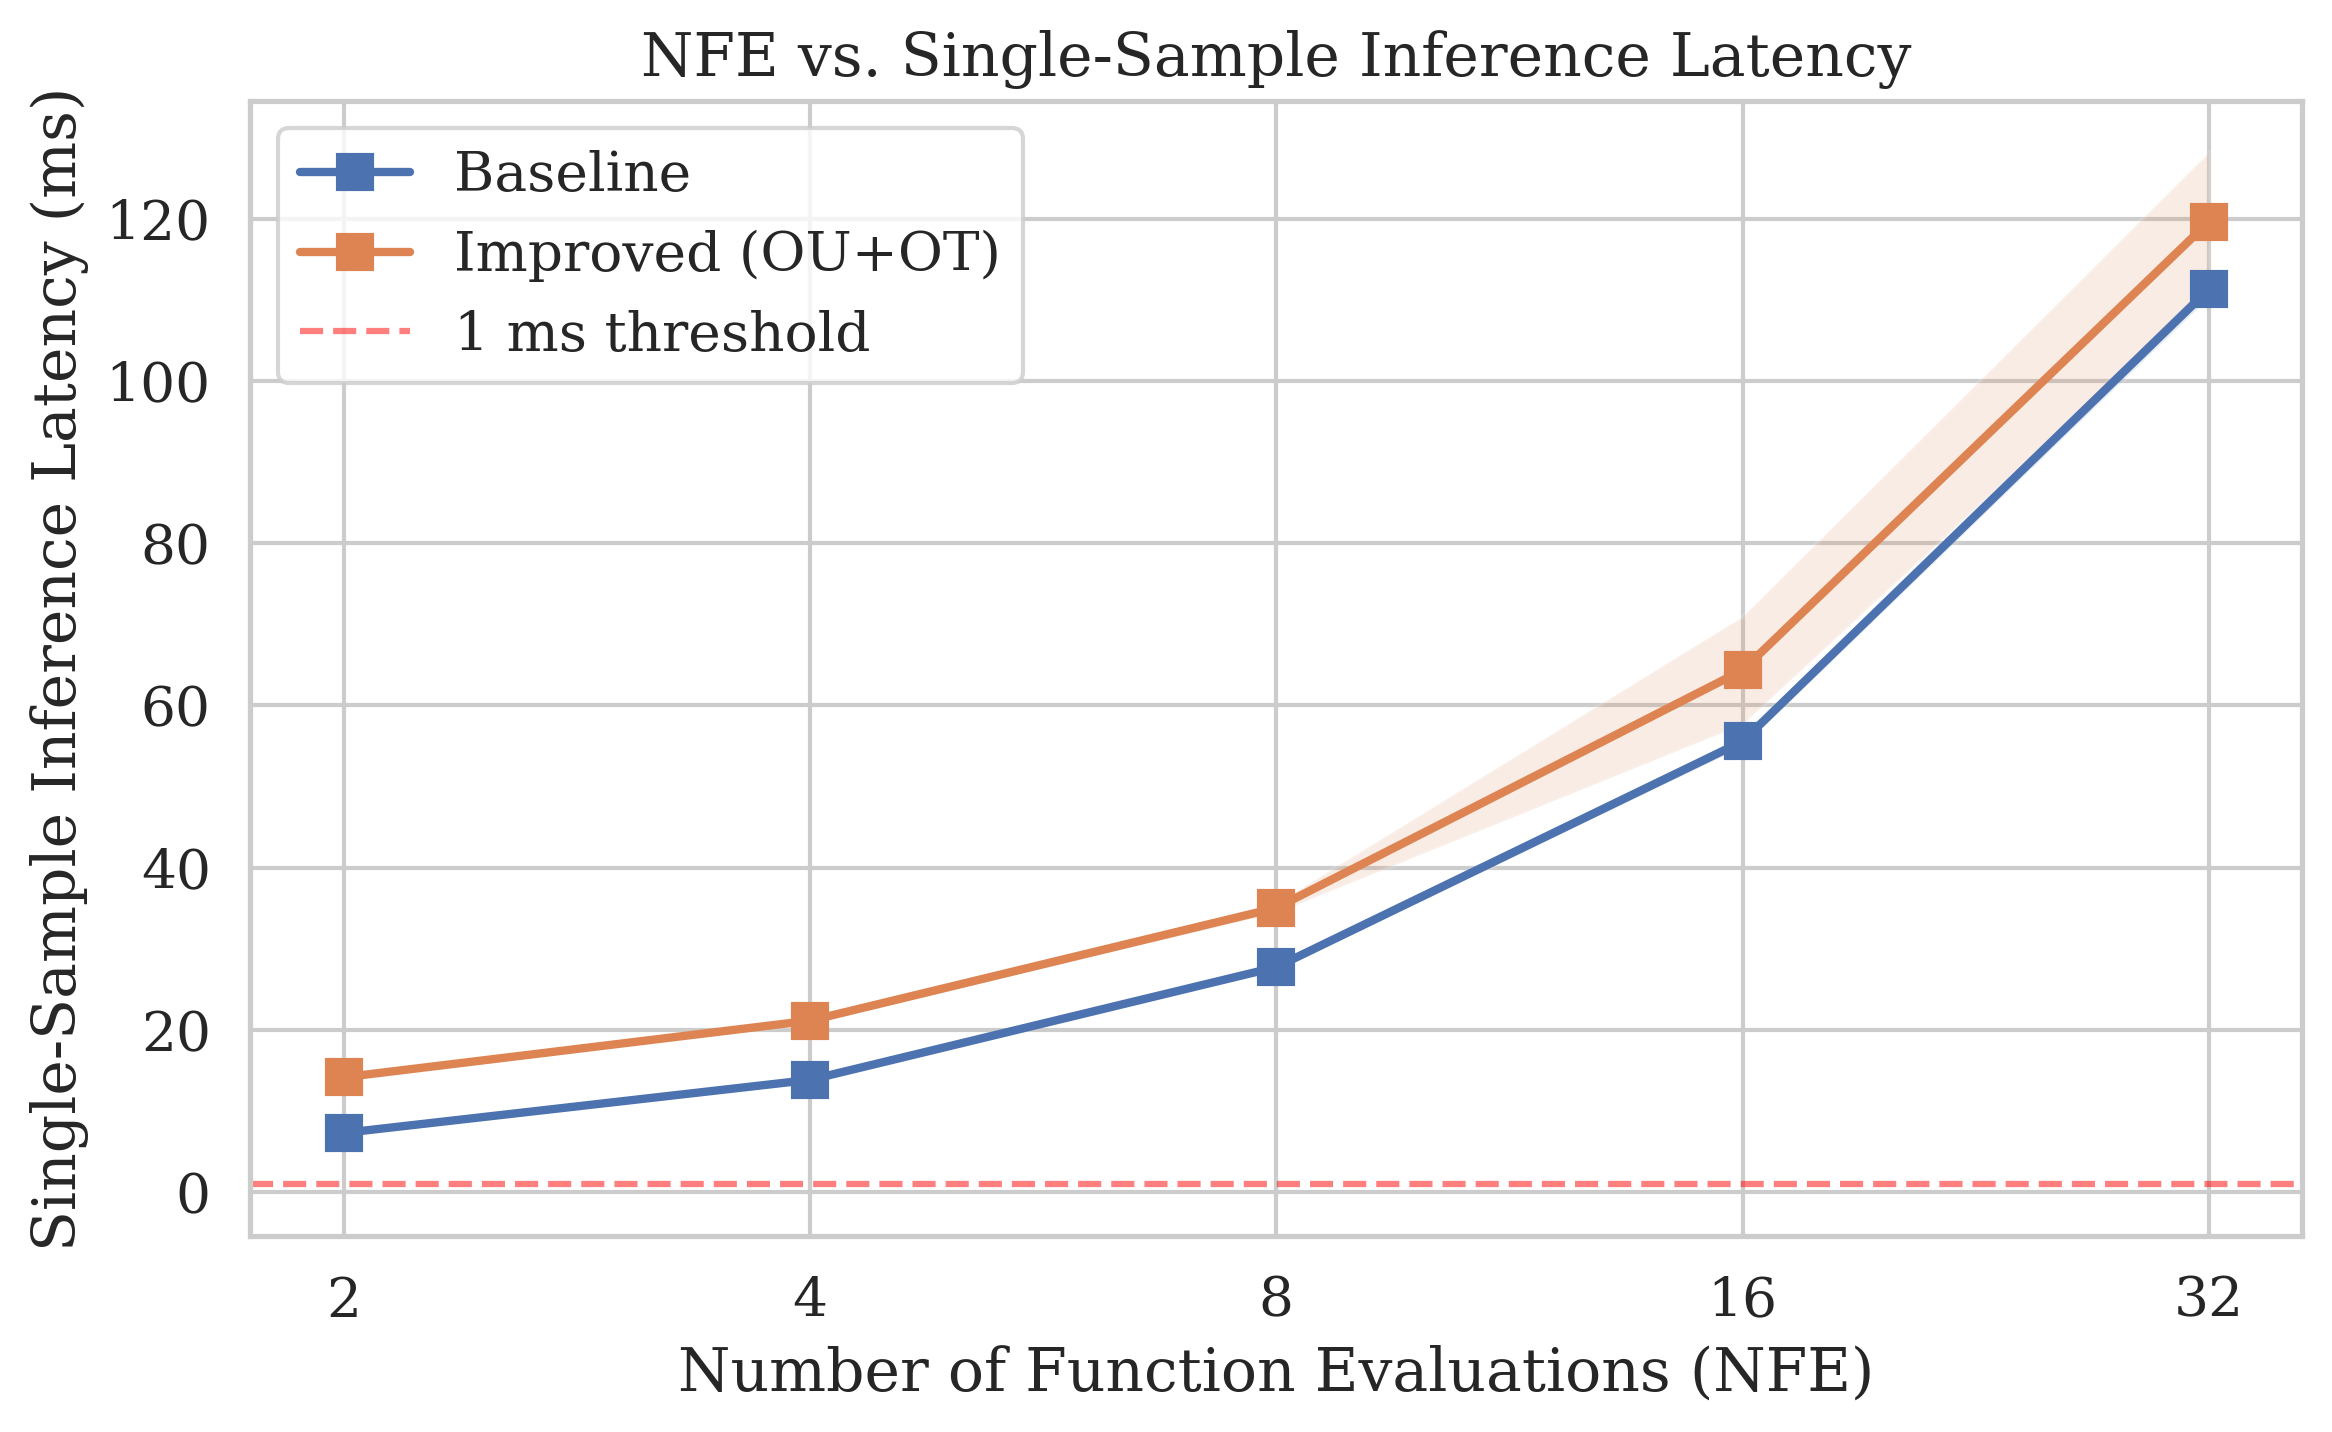
\includegraphics[width=\textwidth]{nfe_vs_latency.png}
    \caption{NFE vs.\ single-sample latency.}
    \label{fig:nfe-latency}
\end{subfigure}
\caption{NFE ablation: accuracy and latency trade-offs.}
\label{fig:nfe-ablation}
\end{figure}

\begin{figure}[H]
\centering
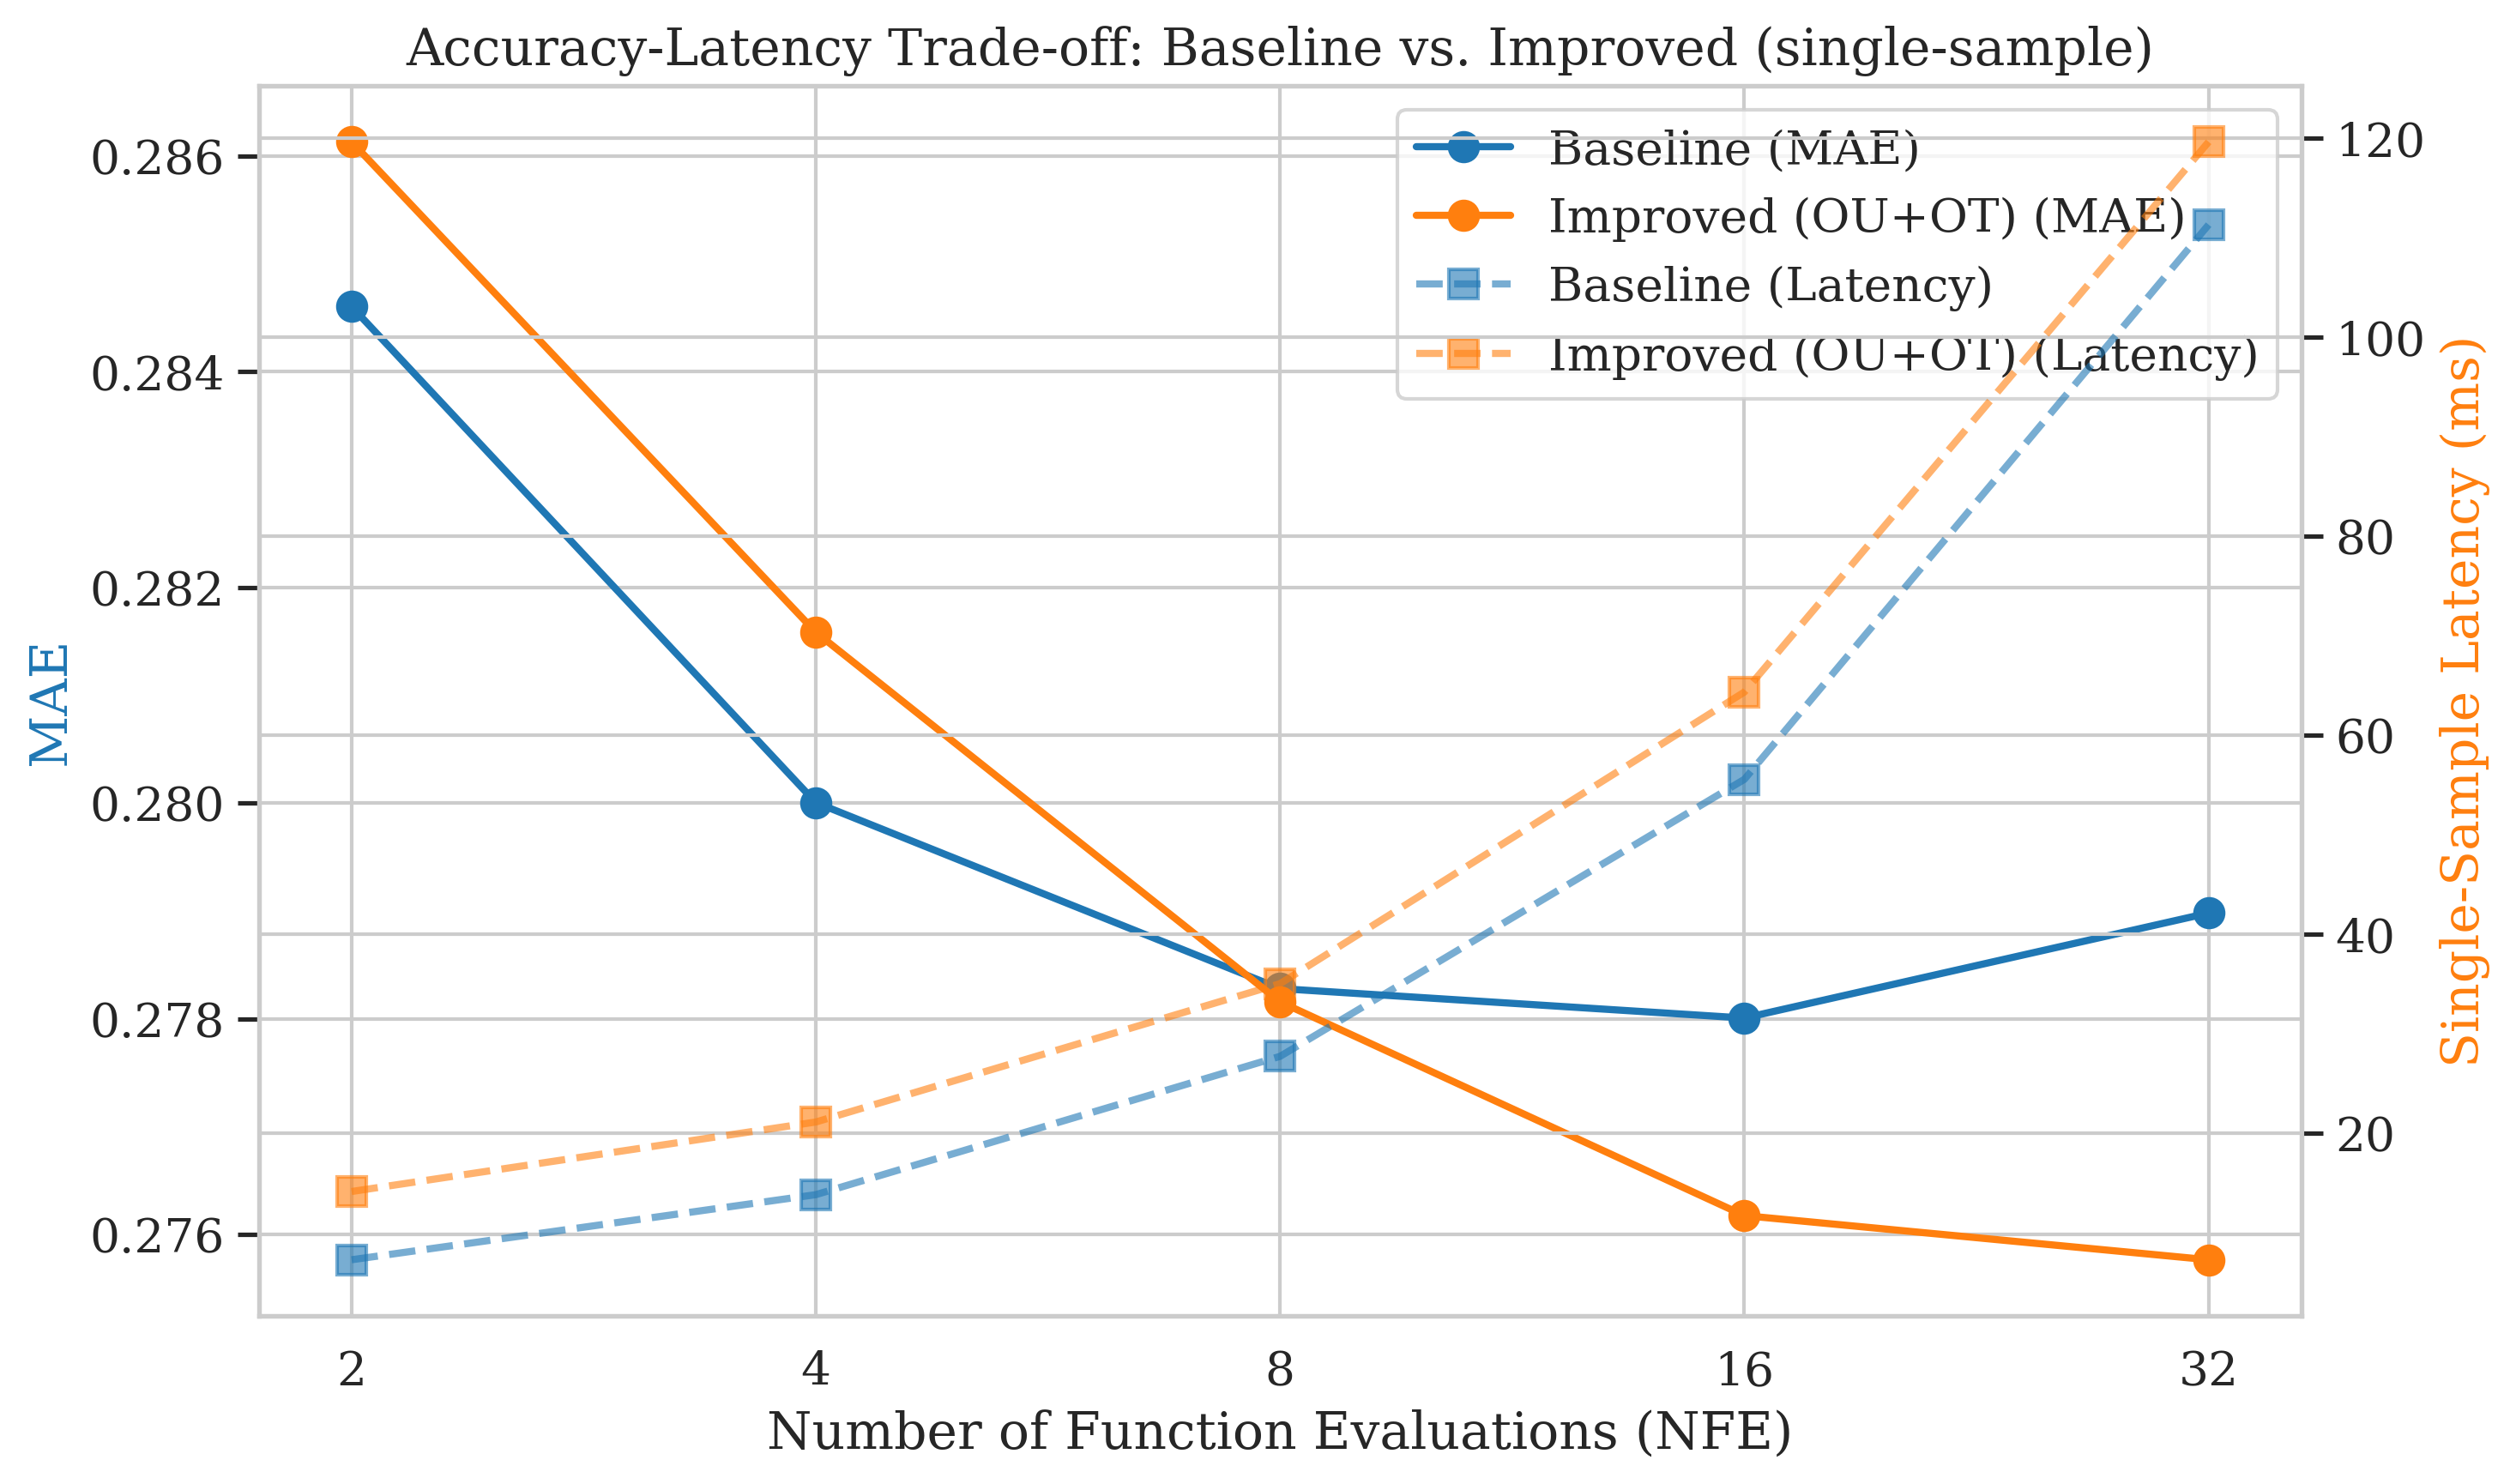
\includegraphics[width=0.7\textwidth]{nfe_accuracy_latency.png}
\caption{Combined accuracy--latency trade-off (dual-axis).
         The improved model at NFE\,=\,4 achieves comparable MAE to the
         baseline at NFE\,=\,16 with \SI{21}{\milli\second} instead of
         \SI{56}{\milli\second} single-sample latency.}
\label{fig:nfe-combined}
\end{figure}

\paragraph{Ablation findings.}

\begin{enumerate}[nosep]
    \item \textbf{Diminishing returns beyond 8~NFEs.}
          Both models show MAE largely plateauing after 8~NFEs.
          The accuracy gain from 8$\to$32 NFEs is less than 0.3\% for both
          models, while latency quadruples.

    \item \textbf{Improved model converges faster.}
          At NFE\,=\,4 the improved model achieves MAE~0.2816---essentially
          matching the baseline's best MAE of~0.2780 at NFE\,=\,16.
          The hypothesis is supported: \emph{the OU\,+\,OT approach requires
          roughly $4\times$~fewer function evaluations for comparable point
          accuracy.}

    \item \textbf{Non-monotonic behaviour at NFE\,=\,32.}
          Both models show slightly \emph{worse} RMSE at NFE\,=\,32 compared
          to NFE\,=\,16 (baseline: 0.652$\to$0.655; improved:
          0.638$\to$0.642).
          This may be due to floating-point accumulation in the fixed-step
          Euler solver combined with float32/AMP precision.

    \item \textbf{Latency overhead of OU prior.}
          The improved model has a constant $\sim$\SI{7}{\milli\second}
          overhead relative to the baseline at each NFE level (e.g.\
          \SI{21.2}{\milli\second} vs.\ \SI{13.9}{\milli\second} at
          NFE\,=\,4).
          This is the cost of sampling from the OU process via
          Euler--Maruyama discretisation at inference time.
\end{enumerate}

% --- Sample predictions ---
\begin{figure}[H]
\centering
\begin{subfigure}[t]{0.48\textwidth}
    \centering
    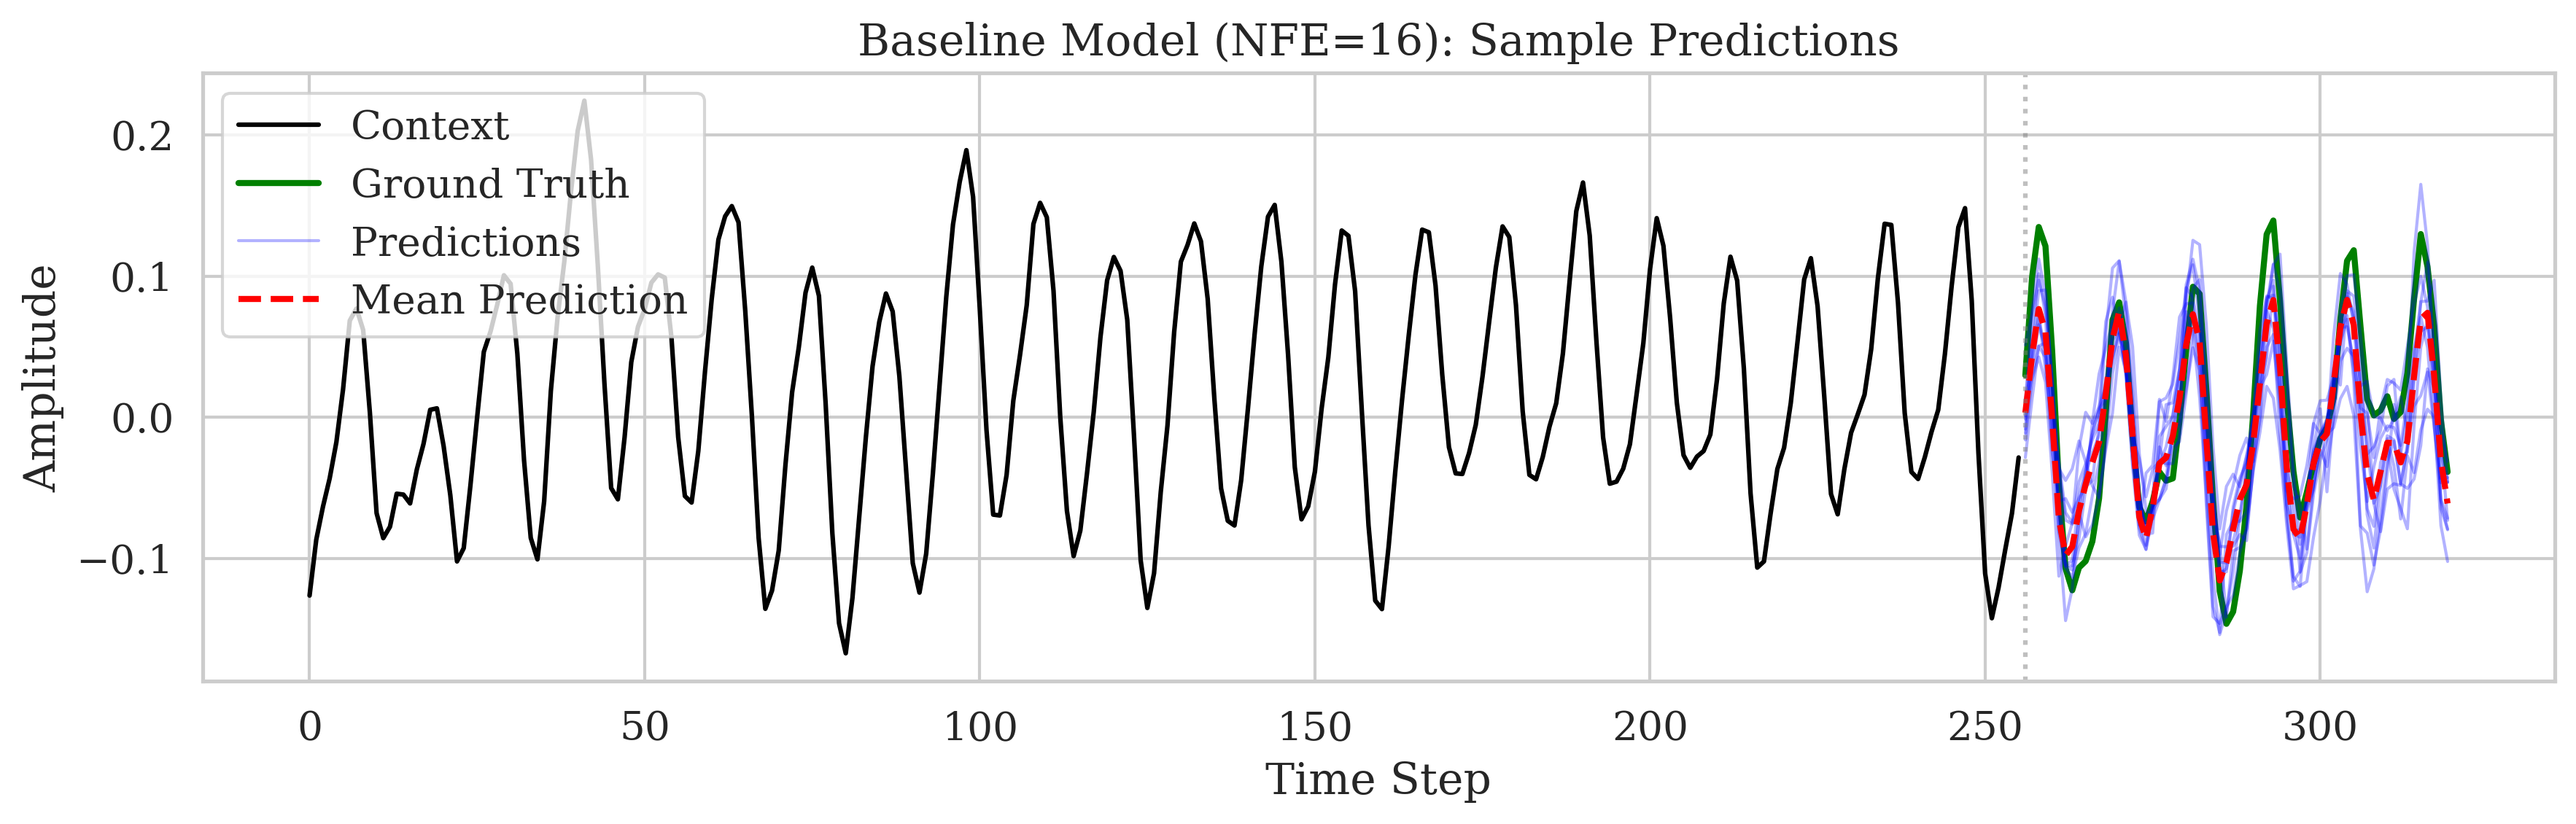
\includegraphics[width=\textwidth]{sample_predictions_baseline.png}
    \caption{Baseline (NFE\,=\,16).}
\end{subfigure}
\hfill
\begin{subfigure}[t]{0.48\textwidth}
    \centering
    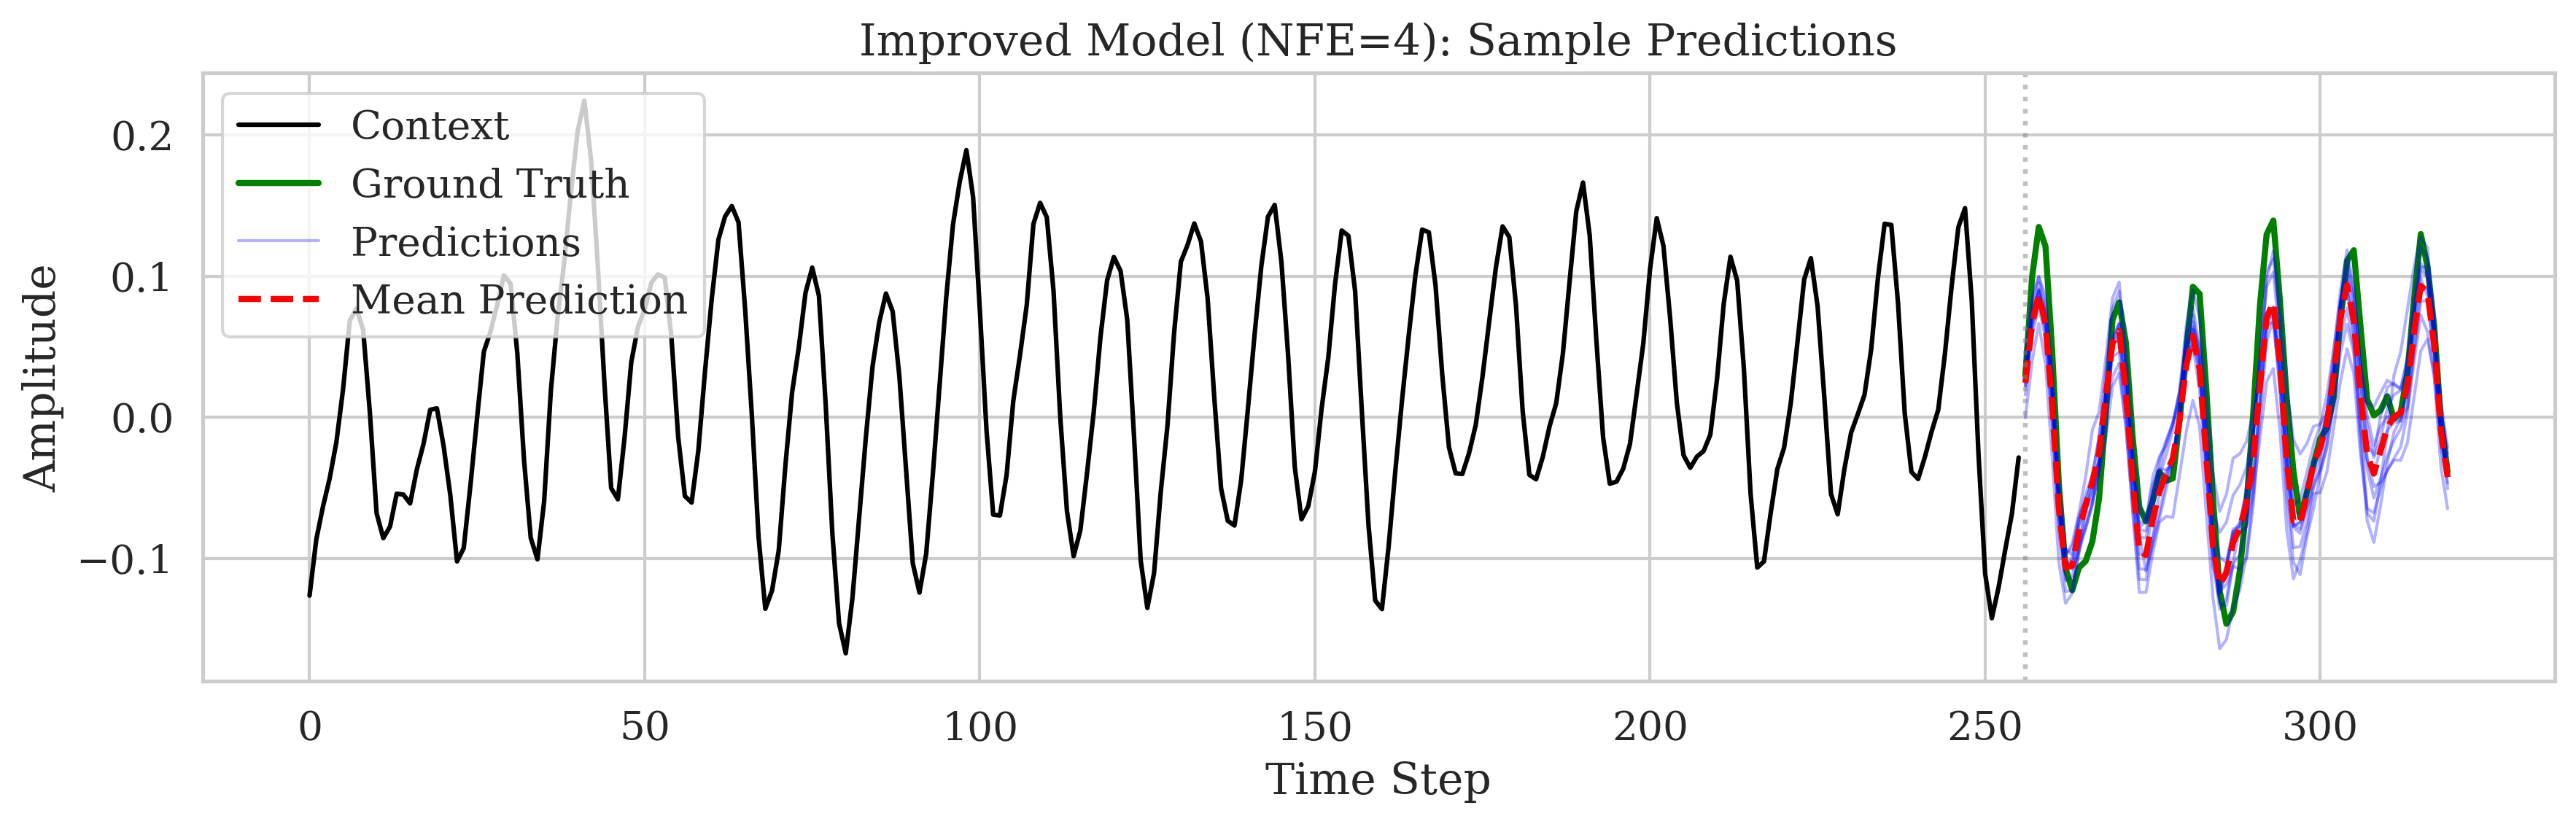
\includegraphics[width=\textwidth]{sample_predictions_improved.png}
    \caption{Improved (NFE\,=\,4).}
\end{subfigure}
\caption{Sample prediction trajectories from the ablation study.}
\label{fig:sample-preds}
\end{figure}

% ==============================================================================
\subsection{Discussion}
\label{sec:discussion}
\textit{(Main Author: Min-Han Yeh)}

\subsubsection{Hypothesis Evaluation}

The central hypothesis---that the improved model at 4~NFEs achieves
competitive MAE/RMSE to the baseline at 16~NFEs---is \textbf{broadly
supported}.
In MAE the gap is under 1\%, and in RMSE the improved model is actually
2.7\% better.
The $3.3\times$ latency reduction from \SI{71}{\milli\second} to
\SI{22}{\milli\second} demonstrates a clear practical benefit.

However, this comes with important caveats.

\subsubsection{The Calibration Trade-Off}

The most significant finding beyond the original hypothesis is the
\textbf{calibration gap}.
The improved model's P10--P90 coverage of 40.5\%
(vs.\ the baseline's 58.5\%) reveals that the OU prior combined with OT
coupling reduces sample diversity during inference.
While this benefits point accuracy by concentrating predictions near the
true signal, it produces overconfident uncertainty estimates.

This is a fundamental consequence of the method: the OU prior generates
temporally correlated noise that is structurally closer to the data than
isotropic Gaussian noise, and the OT coupling during training further reduces
the expected transport distance.
At inference time, different OU noise samples are more similar to each other
than different Gaussian samples would be, leading to tighter---but
underestimating---prediction intervals.

For applications where calibrated uncertainty quantification is critical
(e.g.\ safety-critical systems), this trade-off must be carefully considered.
Neither model achieves the ideal 80\% coverage, suggesting that calibration
improvements (e.g.\ conformal prediction post-processing or increased prior
variance) would be a valuable direction for future work.

\subsubsection{Baseline Overfitting}

The baseline model's training dynamics reveal overfitting from approximately
epoch~50 onward, with validation loss plateauing at $\sim$0.37 while training
loss continued decreasing to $\sim$0.28.
This suggests that the Gaussian prior creates a harder optimisation landscape
for the velocity field: learning to transport unstructured Gaussian noise to
structured time-series data requires the network to encode both temporal
structure and signal dynamics, making it more prone to memorising training
patterns.

In contrast, the improved model's OU prior already encodes temporal
correlations, allowing the velocity field to focus on learning the residual
dynamics.
This results in better generalisation as evidenced by the tight train--val
gap throughout training.

\subsubsection{Practical Implications}

While neither model achieves the sub-millisecond latency target mentioned in
the proposal (a hardware-dependent goal beyond the scope of this project), the
relative improvement is actionable.
In a production setting, the $3.3\times$ speedup could be further amplified
through:

\begin{itemize}[nosep]
    \item Batch inference (amortising overhead across multiple inputs);
    \item Model quantisation (INT8 inference);
    \item Direct deployment on specialised hardware (FPGA/ASIC).
\end{itemize}

The improved model's faster convergence during ODE integration also suggests
potential for adaptive step-size solvers in future work, which could further
reduce the required NFEs.

\end{document}
